	\section{Introduction}


    \begin{frame}{Introducing myself}
        \begin{columns}
            % Column 1
            \begin{column}{0.5\textwidth}
                \begin{itemize}
                    \item Isak Hammer, 27 year old, Lofoten
                    \item Graduate student in Industrial Mathematics
                    \item Research Focus: Analysis and numerical techniques for Partial Differential Equations (PDEs), with a strong emphasis on applications for Finite Element Methods (FEM).
                \end{itemize}
            \end{column}

            % Column 2
            \begin{column}{0.5\textwidth}
                \begin{figure}
                    \centering
                    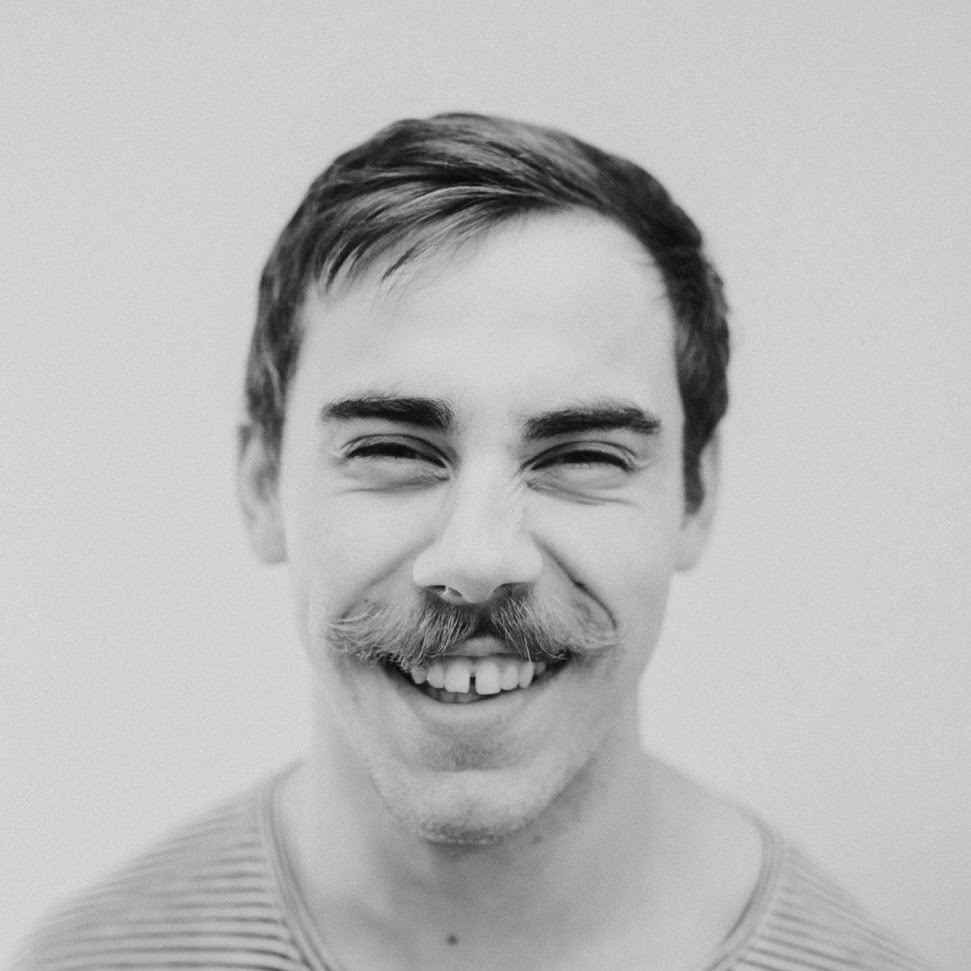
\includegraphics[width=0.7\textwidth]{figures/isak.jpg}
                \end{figure}
            \end{column}
        \end{columns}
    \end{frame}

\begin{frame}{Importance and Motivation of the Cahn Hilliard Equation}
    \begin{columns}
        % Column 1
        \begin{column}{0.5\textwidth}
            \begin{itemize}
            \item Thermodynamically modelling of a two-component liquid separation\footnotemark.
                \item Modelling of so-called lipid rafts in biological membrane dynamics \footnotemark.
            \end{itemize}
        \end{column}
        \begin{column}{0.5\textwidth}
            \begin{itemize}
                \item Droplet dynamics, i.e., coalescence, breakup and movement by coupling with Navier-Stokes \footnotemark.
            \end{itemize}
        \end{column}
    \end{columns}
    \footnotetext[1]{\fullcite{cahn1959free}}
    \footnotetext[2]{\fullcite{yushutin2019computational}}
    \footnotetext[3]{\fullcite{zimmermann2019calculation}}
\end{frame}

\begin{frame}
    \begin{block}{The Cahn Hilliard Equation}
        The general Cahn Hilliard Equation  has the form $u( t,x): \Omega \mapsto [-1,1]   $ s.t.
            \[
            \begin{split}
                 u_t+\Delta\left(\varepsilon \Delta u-\frac{1}{\varepsilon} f(u)\right)&=0 \quad \text{in } \Omega_T:=\Omega \times(0, T) \\
\partial_n u=\partial_n \Delta u& =0 \quad \text{on } \partial \Omega_T:=\partial \Omega \times(0, T) \\
 u & =u_0 \quad \text{on } \Omega \times\{0\}
            \end{split}
            \]
where $f(s)=F^{\prime}(s)$ and $F(s)=\frac{1}{4}\left(s^2-1\right)^2$ and $\Omega \subset \mathbf{R}^d, d=2,3$, is a bounded domain. $\partial_n$ denotes the normal derivative operator on $\partial \Omega$.
\end{block}

\begin{block}{Challenges}
    \begin{enumerate}
        \item Highly nonlinear and stiff. Often the physics require $\varepsilon \ll 1$.
        \item 4th order system.
        \item Conservation of mass and the Neumann conditions conditions.
    \end{enumerate}
\end{block}

\end{frame}



\begin{frame}
\frametitle{Why CutFEM is Well-Suited for the Cahn-Hilliard Equation}

\begin{block}{Cut Finite Element Method (CutFEM)}
    CutFEM is a numerical method for solving partial differential equations (PDEs) using an unfitted mesh.

\begin{figure}
    \centering
    % First TikZ picture
    \begin{minipage}{0.45\textwidth}
        \centering
        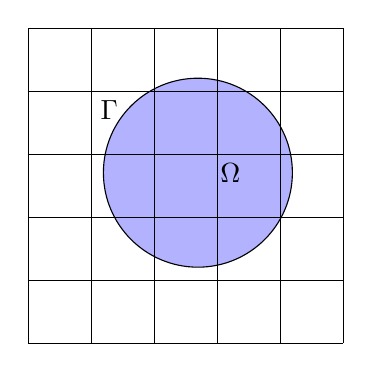
\begin{tikzpicture}[scale=0.80]
            \draw[fill=blue!30] (0.2, 0.2) circle (1.5cm);
            % Background mesh
            \foreach \i in {-2.5, -1.5, ..., 2.5} {
                \draw[line width=0.1pt, shift={(-2.5,\i)}] (0,0) -- (5,0);
                \draw[line width=0.1pt, shift={(\i,-2.5)}] (0,0) -- (0,5);
            }
            % Labels
            \node[below right] at (0.4,0.5) {$\Omega $};
            \node[below right] at (-1.5,1.5) {$\Gamma $};
            % \draw[blue, thick] (-2.5, -2.5) rectangle (2.5, 2.5);
        \end{tikzpicture}
    \end{minipage}
    \hfill
    % Second TikZ picture
    \begin{minipage}{0.45\textwidth}
        \centering
        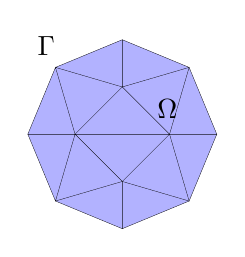
\begin{tikzpicture}[scale=0.80]
            % FIGURE OF UNFITTED MESH
            % Boundary points
            \foreach \i in {0, 45, ..., 315} {
                \coordinate (boundary-\i) at (\i:1.5cm);
            }
            % Interior points
            \coordinate (interior-1) at (0.75, 0);
            \coordinate (interior-2) at (-0.75, 0);
            \coordinate (interior-3) at (0, 0.75);
            \coordinate (interior-4) at (0, -0.75);

            % Create a cycle connecting all the boundary points
            \fill[blue!30] (boundary-0) -- (boundary-45) -- (boundary-90) -- (boundary-135) -- (boundary-180) -- (boundary-225) -- (boundary-270) -- (boundary-315) -- cycle;

            % Labels
            \node[below right] at (0.4,0.7) {$\Omega $};
            \node[below right] at (-1.5,1.7) {$\Gamma $};

            % Triangulation (manually specified)
            \draw[line width=0.1pt] (boundary-0) -- (boundary-45) -- (interior-1) -- cycle;
            \draw[line width=0.1pt] (boundary-45) -- (boundary-90) -- (interior-3) -- cycle;
            \draw[line width=0.1pt] (boundary-90) -- (boundary-135) -- (interior-3) -- cycle;
            \draw[line width=0.1pt] (boundary-135) -- (boundary-180) -- (interior-2) -- cycle;
            \draw[line width=0.1pt] (boundary-180) -- (boundary-225) -- (interior-2) -- cycle;
            \draw[line width=0.1pt] (boundary-225) -- (boundary-270) -- (interior-4) -- cycle;
            \draw[line width=0.1pt] (boundary-270) -- (boundary-315) -- (interior-4) -- cycle;
            \draw[line width=0.1pt] (boundary-315) -- (boundary-0) -- (interior-1) -- cycle;

            % Triangulation between interior points
            \draw[line width=0.1pt] (interior-1) -- (interior-2) -- (interior-3) -- cycle;
            \draw[line width=0.1pt] (interior-1) -- (interior-2) -- (interior-4) -- cycle;

            % \draw[blue, thick] (-2.5, -2.5) rectangle (2.5, 2.5);

        \end{tikzpicture}
    \end{minipage}
\caption{Examples fitted mesh and a unfitted mesh for a circle.}
\label{fig:domain_mesh}
\end{figure}

\end{block}

\end{frame}
